\documentclass[t]{beamer}
\usetheme{Madrid}
\usecolortheme{seahorse}
\definecolor{seahorse}{RGB}{189, 186, 238}
\setbeamercolor{block title}{bg=seahorse,fg=black}

\usepackage{multicol}
\usepackage{tikz}
\usepackage{amsmath}
\usepackage{amssymb}
\usepackage{tcolorbox}
\usepackage{mathtools}
\usepackage{mathrsfs}
\usepackage{physics}
\usepackage{bm}
\usepackage{bbm}
\usepackage[export]{adjustbox}


\title{Error bounds for numerical approximations}
\author[MAT264] 
{Kaja Jurak, Esther Jerez}

\institute[UIB]
{
	Faculty of Mathematics\\
	University of Bergen
	
}
\date[2021]
{May 2021}


\logo{
	\begin{tikzpicture}
	\node[inner sep=0pt] (logo) at (0,0)
	{
\includegraphics[width=.25\textwidth]{uiblogo.png}};
	\end{tikzpicture}}


\setlength\parindent{0pt}
\begin{document}
	\frame{\titlepage}
	\begin{frame}
	\frametitle{Introduction}
	Our main goal is to give accurate error bounds for approximated solutions of a PDE. In concrete, we will focus on the problem of the steady-state heat equation, described by  \alert{Poisson's equation}:
	\begin{align*}
	\bm{q} = -k \nabla ^2 u
	\end{align*}
	where 
	\begin{enumerate}
		\item[] $\bm{q}$ is the heat flux,
		\item[] $k$ is the materials' thermal conductivity,
		\item[] $u$ is the temperature.
	\end{enumerate}
	With the previous PDE we will look at the flow rates or fluxes of energy locally. \\
	
	% \begin{block}{Remark}
	%     Sample text
	% \end{block}
	
\end{frame}

\begin{frame}
\frametitle{Introduction}
\begin{columns}[t]
	\column{0.5\textwidth}
	\textbf{1D CASE}
	\begin{align*}
	&\frac{\partial q}{\partial x} = f \\
	&q = -k \frac{\partial u}{\partial x} 
	\end{align*}
	And we will consider the following situations:
	\begin{itemize}
		\item[1.] Linear flux ($\frac{\partial q}{\partial x} = 1$) and constant thermal conductivity ($k=1$).
		\item[2.] Non-linear flux and non-constant thermal conductivity
	\end{itemize}
	
	\column{0.5\textwidth}
	\textbf{2D CASE} \\
	\begin{align*}
	\frac{\partial q_1}{\partial x} + \frac{\partial q_2}{\partial y}  &= f \\
	\bm{q} = (q_1,\; q_2)^T  &= -k \left( \frac{\partial T}{\partial x} ,\; \frac{\partial T}{\partial y}\right)^T
	\end{align*}
	Here we will consider a final problem where both $f$ and $k$ are more complex function, but we do know the real solution.
\end{columns}        
\end{frame}

\begin{frame}
\frametitle{Error bounds computations}
We are considering a general elliptic PDE:
\begin{align*}
\nabla q = f , \quad q =-k \nabla u
\end{align*}
Main idea: instead of measuring $\norm*{u-v} = \norm*{e_v}$, study $\norm*{k^{\frac{1}{2}}\nabla e_v}$. 
\\ By integrating the PDE and some more computations we obtain:
\begin{align*}
\norm*{k^{\frac{1}{2}}\nabla e:v} \leq \norm*{k^{-\frac{1}{2}}(\bm{r}+k\nabla v)} + C_{\Omega,k}\norm*{f-\nabla \bm{r}} \equiv \mathcal{M}(v,r;f)
\end{align*}
where $\bm{r}$ is an approximation to the flux function.
With this error bound, we will also consider the \alert{relative error}:
\begin{align*}
\frac{\norm*{k^{\frac{1}{2}}\nabla e_v}}{\norm*{k^{\frac{1}{2}}\nabla v}} \leq \frac{\mathcal{M}(v,r;f)}{\norm*{k^{\frac{1}{2}}\nabla v}}
\end{align*}

\end{frame}

\begin{frame}
\frametitle{Error bounds computations}
When we do know the the real solution, we will also compute the \alert{efficiency index of the potential}:
\begin{align*}
I^{eff}_v = \frac{\mathcal{M}(v,r;f)}{\norm*{k^{\frac{1}{2}}\nabla e_v}}
\end{align*}
Combining the energy errors of both the potential and the flux:
\begin{align*}
\norm*{(e_v,e_r)}_{*} \equiv \norm*{k^{\frac{1}{2}}\nabla e_v} + \norm*{k^{-\frac{1}{2}}e_r} + C_{\Omega,k}\norm*{\nabla e_r}
\end{align*} 
And indeed, we can prove with the previous concepts that 
\begin{align*}
\mathcal{M}(v,r;f) \leq  \norm*{(e_v,e_r)}_{*}  \leq 3\mathcal{M}(v,r;f)
\end{align*}
respectively
\begin{align*}
1 \leq I^{eff}_{v;r} = \frac{3\mathcal{M}(v,r;f)}{\norm*{(e_v, e_r)}_*} \leq 3
\end{align*}
\end{frame}

\begin{frame}
\frametitle{Error bounds computations}
Also, if we consider the definition of the Poincaré constant:
\begin{align*}
C_{\omega,k} \equiv \mathrm{sup}_e \frac{\norm*{e}}{\norm*{k^{\frac{1}{2}}\nabla{e}}}
\end{align*}
We can obtain that for any function $e$ it always will hold:
\begin{align*}
\norm*{e} \leq C_{\Omega,k}\norm*{k^{\frac{1}{2}}\nabla{e}} \leq C_{\Omega,k}\mathcal{M}(v,r;f)
\end{align*}
\end{frame}

\begin{frame}
\frametitle{Implementation of the method}
\begin{multicols}{2}[\columnsep2em] 
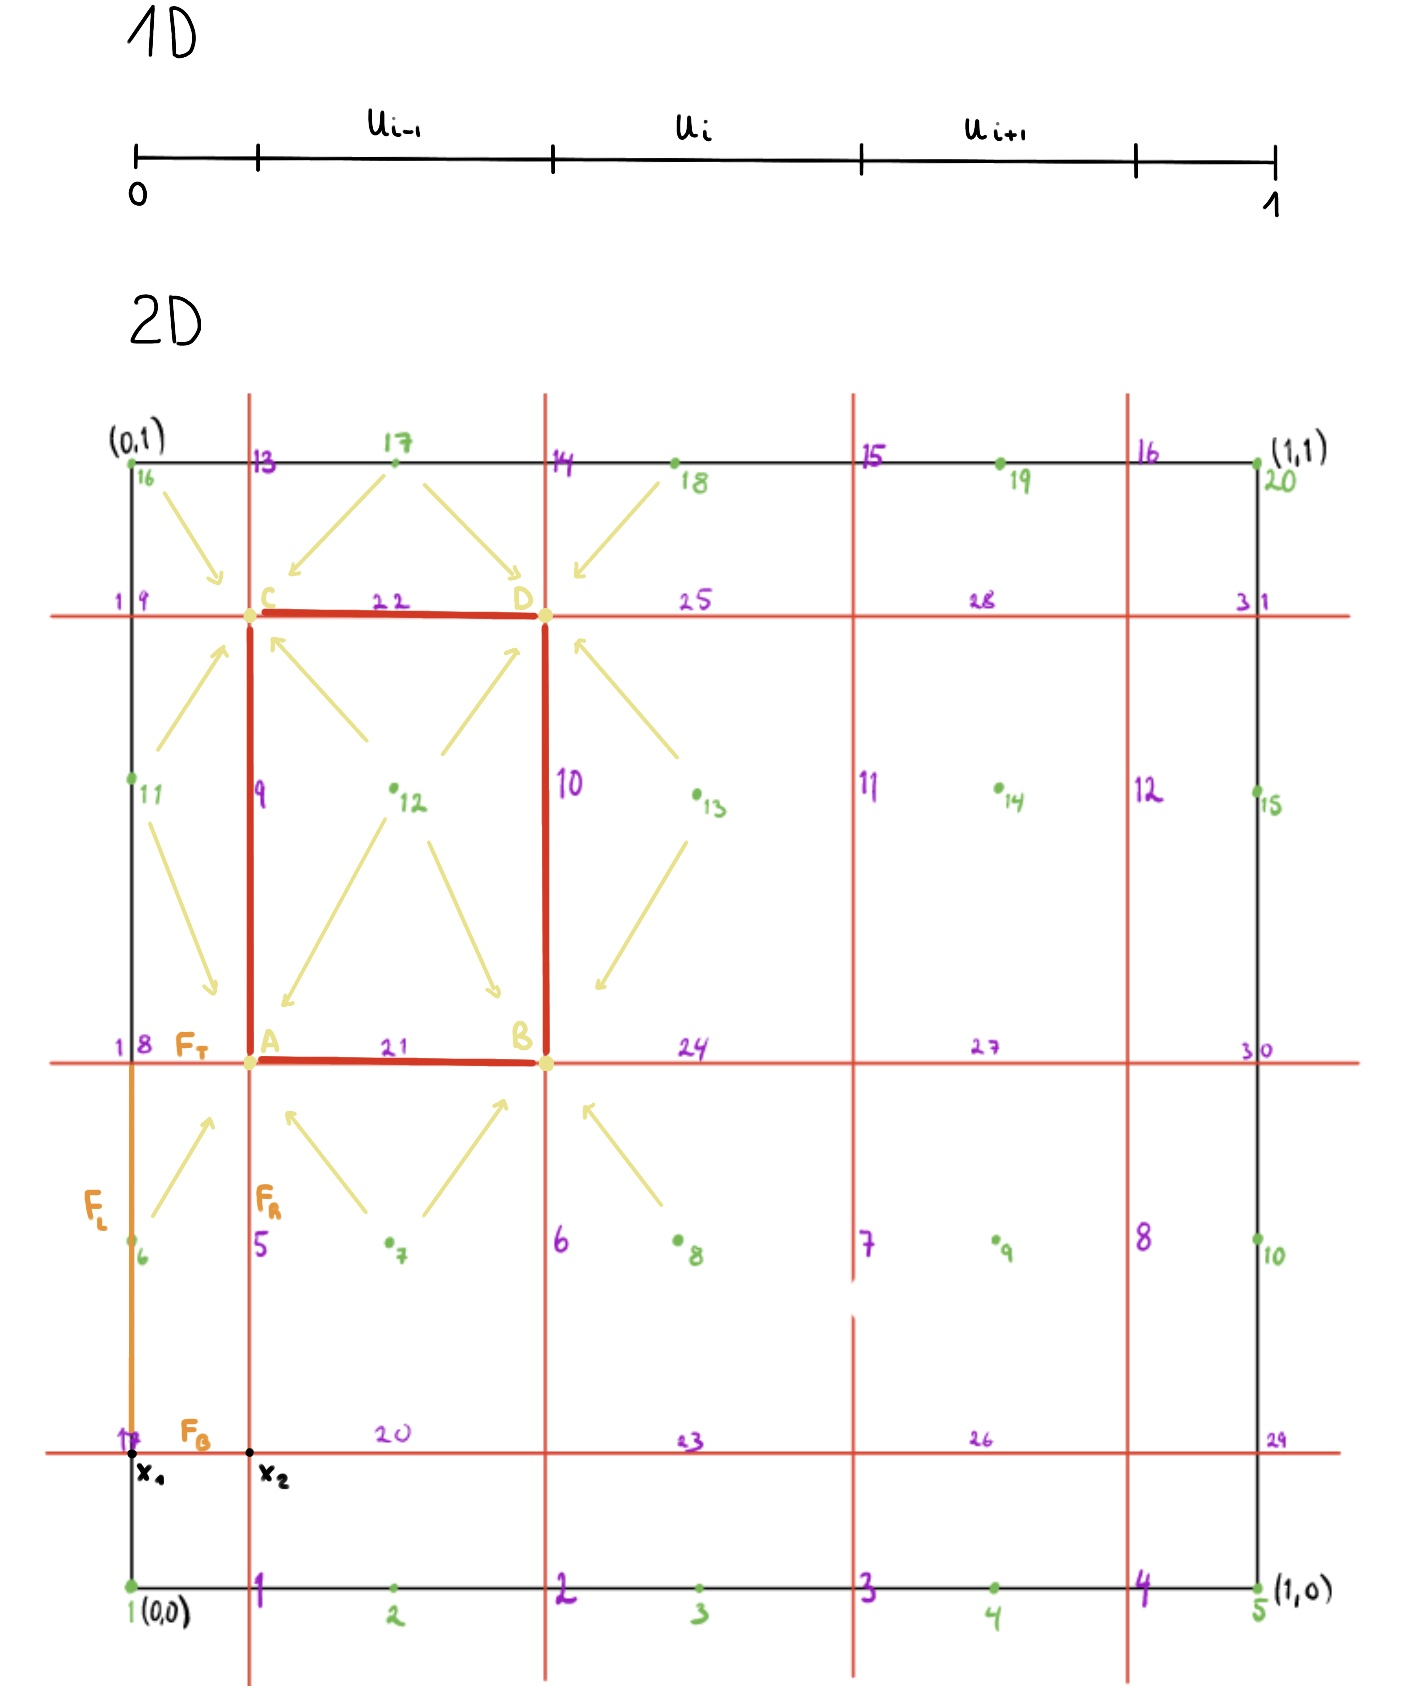
\includegraphics[width=\linewidth]{square.jpg}
\columnbreak
\begin{itemize}
\item For each cell, we will approximate the potential ($v_h \approx u$)
\item flux satisfies an integral form of conservation, so we can compute the flux ($r_h$) in every edge surrounding the cell using finite difference.
\item Interpolating both flux and potential we can then obtain functions smooth enough to work with them. 
\end{itemize}

\end{multicols}

\end{frame}

\begin{frame}
\frametitle{Implementation of the method}

If we are considering the 1D case, following the conservation law for cell $i$ we have:
\begin{align*}
q_{i+1} - q_i =  \int_{w_i} f
\end{align*}

This can be applied the same way in the 2D case, component by component. For the particular case of a left side cell we would compute the flux on the left edge by:
\begin{align*}
F_L &= F_R - \int\limits_{x_1}^{x_2} f(x,y) \,dx\ \\
&=  F_R - f(x,y)\Delta x \quad \text{\scriptsize{(Cause we are considering f being constant)}}
\end{align*}
\end{frame}

\begin{frame}
\frametitle{Results in 1D - $k,f$ constant}
%\begin{minipage}{0.8\textwidth}
\vspace{-18pt}
\begin{figure}[t]
%\centering
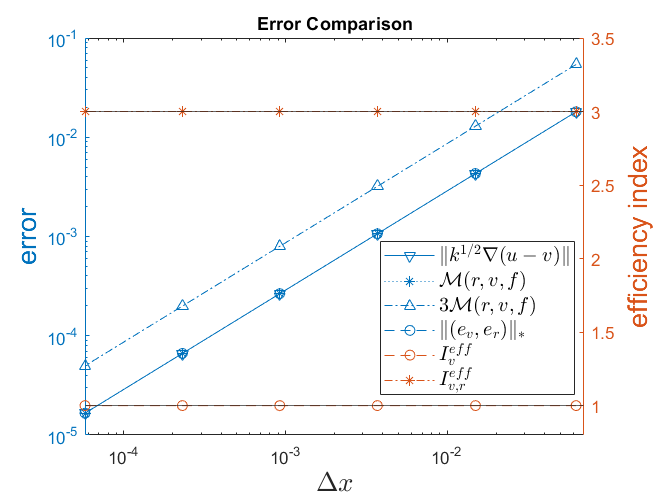
\includegraphics[width = 0.7\linewidth]{convergenceplot_k_f_constant.png}
\caption{Poisson equation in 1D with conductivity $k(x) = 1$ and heat source $f(x) = 1$.}
\label{fig:Convergence1d1}
\end{figure}
\end{frame}

\begin{frame}{Result 1D - $k$ non-constant, $f$ non-linear}
\begin{figure}
\vspace{-5pt}
\centering
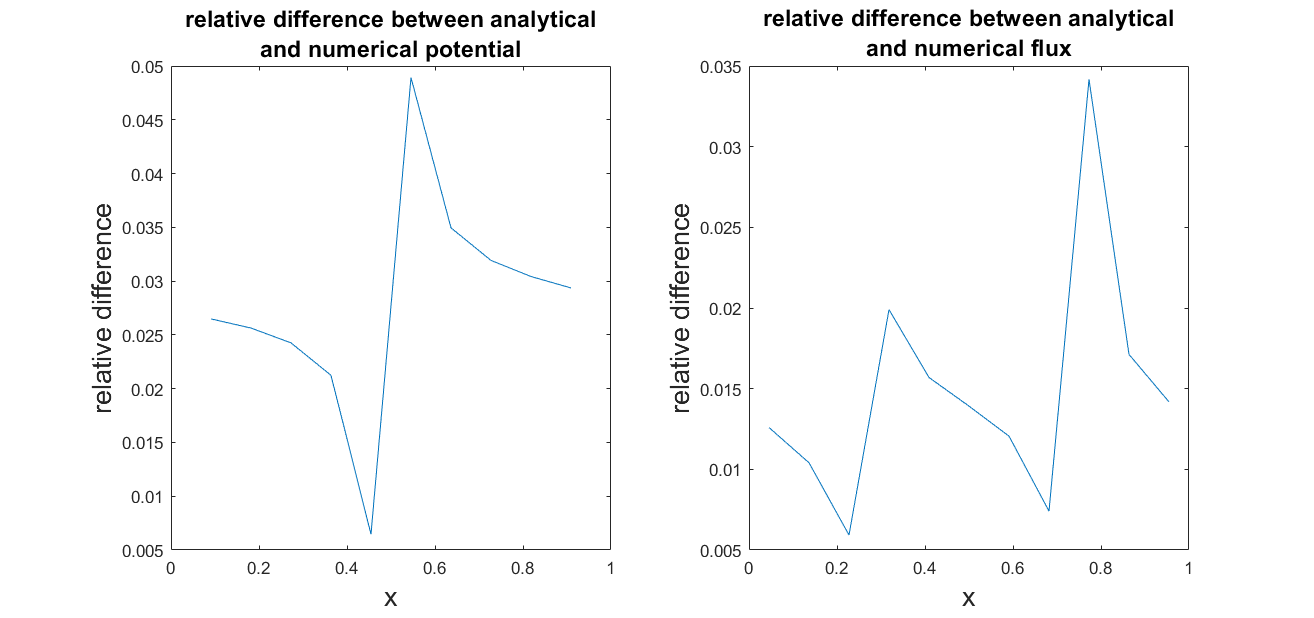
\includegraphics[width = 1.0\linewidth, left]{difference_analytical_numerical.png}
\caption{Relative difference between analytical and numerical solution of Poisson equation with $k(x) = 2-x$ and $f(x) = 4\pi^2\sin(2\pi x)\cdot k(x) + 2\pi\cos(2\pi x)$.}
\label{fig:fig:diff}
\end{figure}
\end{frame}

\begin{frame}
\frametitle{Results in 1D - $k$ non-constant, $f$ non-linear}
%\begin{minipage}{0.8\textwidth}
\vspace{-18pt}
\begin{figure}[t]
\centering
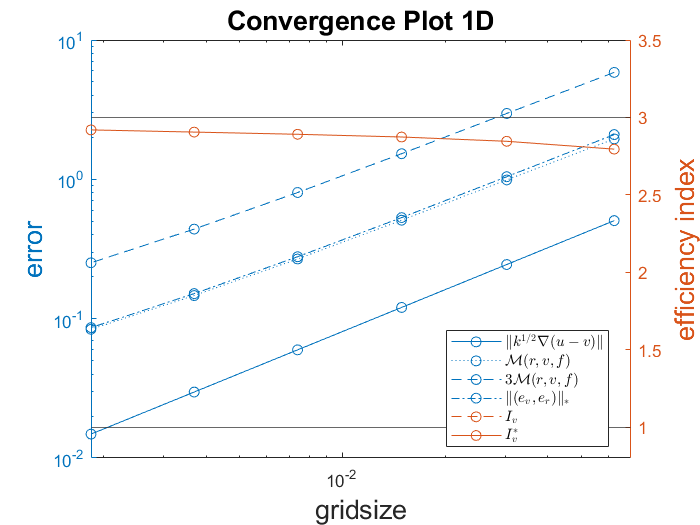
\includegraphics[width = 0.7\linewidth]{convergenceplot_k_f_non_constant.png}
\caption{Poisson equation in 1D with conductivity $k(x) = 2-x$ and heat source $f(x) = 4\pi^2\sin(2\pi x)\cdot k(x) + 2\pi\cos(2\pi x)$.}
\label{fig:Convergence1d}
\end{figure}

% \end{minipage}
\end{frame}

\begin{frame}
\frametitle{Results in 2D}
\begin{figure}
\centering
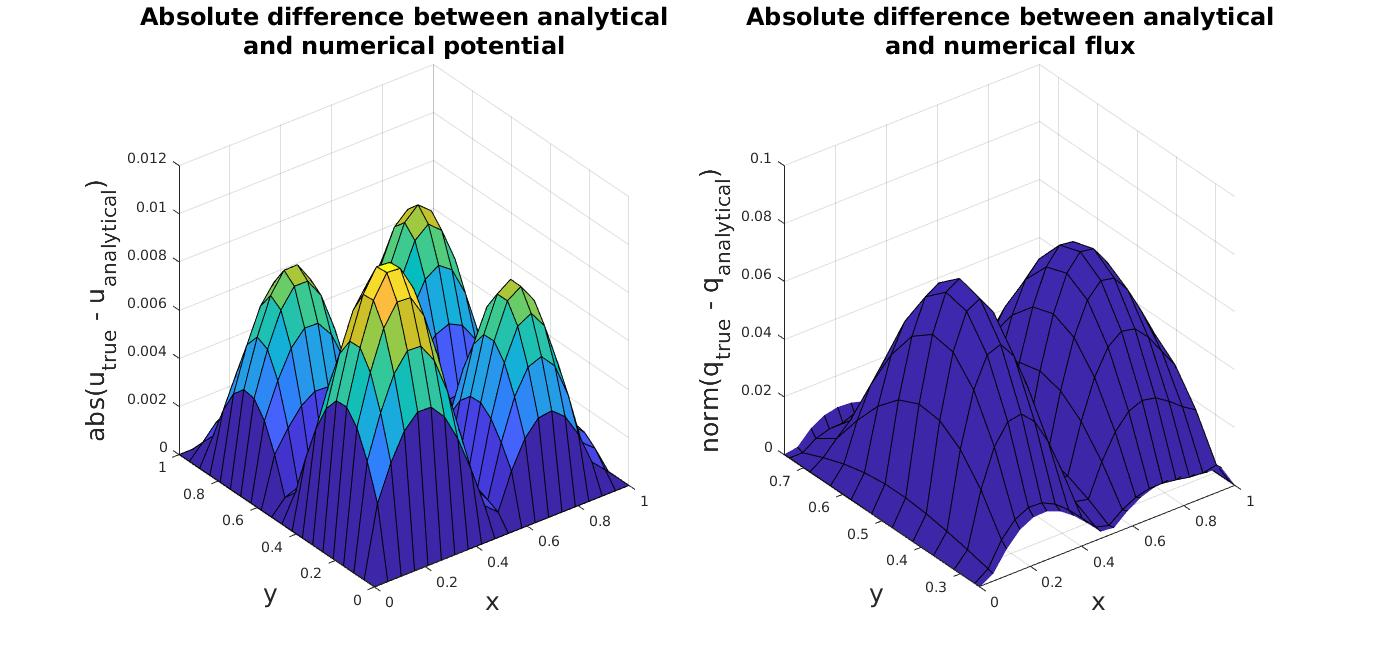
\includegraphics[width = 0.9\linewidth]{../../Images/absnorm.jpg}
\caption{$f(x,y) = 8\pi^2\sin{2\pi x}\sin{2\pi y}k(x,y) - 2\pi\cos{2\pi x}\sin{2\pi y}(y-1)$ $+ 2\pi\sin{2\pi x}\cos{2\pi y}(x-1) $ and 
$k(x,y) = 1 + (x-1)(y-1)$}
\end{figure}	
\end{frame}

\begin{frame}[c]
\frametitle{Results in 2D}
\begin{table}[c]
\begin{tabular}{c | c | c | c | c | c } 
$\zeta$ & $\mathcal{M}$  & $\norm*{k^{\frac{1}{2}}\nabla e_v}$ & $\norm*{(e_v,e_r)}_{*}$ & $I_v^{eff}$ & $I_{v,r}^{eff}$ \\
\hline \hline
$\zeta_1$ & 2.61 & 6.36e-1 & 2.99 & 4.10 & 2.62 \\ 
$\zeta_2$ & 1.25 & 2.95e-1 & 1.43 & 4.26 & 2.63 \\
$\zeta_3$ & 6.19e-1 & 1.43e-1& 7.03e-1 & 4.31 & 2.64 \\
$\zeta_4$ & 3.07e-1 & 7.10e-2 & 3.48e-1 & 4.32 & 2.64 \\
\end{tabular}
\caption{$f(x,y) = 8\pi^2\sin{2\pi x}\sin{2\pi y}k(x,y) - 2\pi\cos{2\pi x}\sin{2\pi y}(y-1)$ $+ 2\pi\sin{2\pi x}\cos{2\pi y}(x-1) $ and 
$k(x,y) = 1 + (x-1)(y-1)$ with a grid refinement of $2^4$.}
\end{table}

\end{frame}

\begin{frame}
\frametitle{Results in 2D}
\begin{figure}
\centering
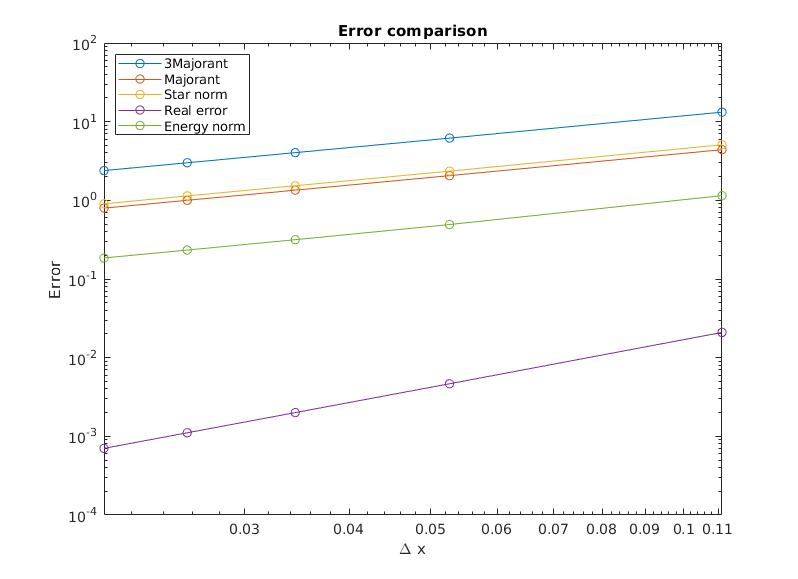
\includegraphics[width = 0.7\linewidth]{../../Images/errorcomparison2d.jpg}
\caption{$f(x,y) = 8\pi^2\sin{2\pi x}\sin{2\pi y}k(x,y) - 2\pi\cos{2\pi x}\sin{2\pi y}(y-1)$ $+ 2\pi\sin{2\pi x}\cos{2\pi y}(x-1) $ and 
$k(x,y) = 1 + (x-1)(y-1)$}
\end{figure}
\end{frame}

\begin{frame}
\frametitle{Conclusion}
\begin{itemize}
\item The Runge-Kutta estimate gives an upper bound, but we do not know how far away the real error can be.
\item We are able to bound the combined energy-norm from below and above \textit{without knowing} the real solution.
\item After testing the method with problems where we know the true solution, we can trust it for problems with an unknown solution.
\end{itemize}
\end{frame}

\begin{frame}
\frametitle{References}
\begin{enumerate}
\item[I] Lecture Notes Mat264: Computational Science II, Univisersitet i Bergen, Jan Nordbotten, Spring Semester 2021.
\item[II] Matlab files from Erlend.
\item[III]  \href{https://en.wikipedia.org/wiki/Heat_equation\#Specific_examples}{Wikipedia Heat equation}
\end{enumerate}
\end{frame}

\end{document}
